\chapter{On the Power of Small Toric Codes} 
\label{ch:SurfaceCodes}

\section{Introduction to the Toric Code}


Toric code simple
Excellent local 

Other operations

Other codes

In this chapter we look towards an experimental realisation of the toric code and study the code for small values of $n$. We pre-compute a decoding library, an approach that quickly becomes intractible for values of $n$ above those considered here, but has the advantage that we obtain a provably optimum decoding success rate. We use our pre-computed decoder to assess the \textit{encoding power} of the code: we say the code has positive encoding power if the encoded qubits exhibit a lower error rate than the same number of unencoded qubits subjected to the same noise.

\subsection{Revisiting Shor's code}

First consider a simple code. The first stage of Shor's code.

\begin{align}\label{shor_state}
  \alpha\ket{0} + \beta\ket{1} \rightarrow \alpha\ket{000} + \beta\ket{111}
\end{align}

Introduce the qubit operators as in the quantum literature
\begin{align}
  Z &= \ket{0}\bra{0} - \ket{1}\bra{1} \\
  X &= \ket{0}\bra{1} + \ket{1}\bra{0} \\
  Y &= \ket{0}\bra{1} - \ket{1}\bra{0} = ZX
\end{align}

Notice that the operators $Z_1 Z_2$, $Z_2 Z_3$ and $Z_1 Z_3$ all leave $\ket{\psi}$ unchanged. As these operators commute we can find states which are simultaneous eigenstates of all three. 
\begin{figure}\label{ops_states}
  \begin{center}
    \begin{tabular}{c c c c c}
      State & $Z_1 Z_2$ & $Z_2 Z_3$ & $Z_1 Z_3$ & $Z_1$ \\
      \hline
      $\ket{000}$ & $+1$ & $+1$ & $+1$ & $+1$ \\
      $\ket{001}$ & $+1$ & $-1$ & $-1$ & $+1$ \\
      $\ket{010}$ & $-1$ & $-1$ & $+1$ & $+1$ \\
      $\ket{100}$ & $-1$ & $+1$ & $-1$ & $-1$ \\
      $\ket{110}$ & $+1$ & $-1$ & $-1$ & $-1$ \\
      $\ket{101}$ & $-1$ & $-1$ & $+1$ & $-1$ \\
      $\ket{011}$ & $-1$ & $+1$ & $-1$ & $+1$ \\
      $\ket{111}$ & $+1$ & $+1$ & $+1$ & $-1$
    \end{tabular}
  \end{center}
  \caption{The eigenvalues of the operators on their simultaneous eigenstates}
\end{figure}

\begin{align}
  (Z_1Z_2)(Z_2Z_3) = Z_1Z_3
\end{align}
The operators are not independent. The eigenvalue of the third can be inferred from the other two.

The set $\{Z_1Z_2, Z_2Z_3, Z_1\}$ is independent. The eigenvalues of these operators uniquely define the basis states. Call these stabilisers of the state $\ket{000}$. Similarly $\{Z_1Z_2, -Z_2Z_3, Z_1\}$ would stabilise $\ket{001}$.

Taking $\{Z_1Z_2, Z_2Z_3\}$ uniquely defines a subspace spanned by $\{\ket{000}, \ket{111}\}$ - precisely the codespace defined in Eqn. (\ref{shor_state}). Repeated measurement would give the same result.


The operator on the logical qubit can be taken to be $Z_1$. 

Errors can be taken to be the $X$ and $Z$ acting on each qubit. To take a concrete example consider $X_1$ acting on the state.
\begin{align}
  X_1 (\alpha\ket{000} + \beta\ket{111}) = \alpha\ket{100} + \beta\ket{011}
\end{align}
If we evaluate the stabilisers now we find $Z_1Z_2 \rightarrow -1$ and $Z_2 Z_3 \rightarrow +1$. We know that an error has occurred. Can predict these outcomes by noticing that $(Z_1Z_2)X_1 = -X_1(Z_1Z_2)$. The outcome of our stabiliser has now changed. We can tell an error has taken place. We do not know if it was $X_1$ or $X_2X_3$. In Shor's scheme we correct the most likely. A different way of looking at this is that we can return to the codespace by applying $X_1$: if the error was actually $X_1$ the logical qubit will be intact, but if the error was $X_2X_3$ the overall operation will be $X_1X_2X_3$ and there will be an error on the logical qubit.

If we instead have a phase flip $Z_1$ we will not be able to detect this as it commutes with the stabilisers and will go unseen. In Shor's original paper he fixes this by expanding the codespace.

We have introduced the stabiliser notation to describe a familiar code. We have seen how by measuring stabiliser operators we can detect certain errors. We have an operator that completes the commuting set that defines an operation on the logical qubit. We will now use this language to introduce the toric code.

\subsection{Definition of Toric Codespace}

The toric $2n$-code (Fig. \ref{4-code}) uses $2n^2$ physical qubits to encode $2$ logical qubits. The \textit{codespace}, the subspace  that the code states inhabit, is most elegantly described using the \textit{stabiliser formalism} - by specifying a set of commuting operators with respect to which the state is invariant. In particular, in a $2^n$ dimensional Hilbert space by specifiying a set of $n$, independent, commuting, binary-outcome operators we uniquely determine the state. 

To describe the code, it is useful to picture the $2n^2$ physical qubits positioned on the odd diagonals of a $2n \times 2n$ lattice (i.e. in the positions with coordinates $(i,j)$, where $i+j$ is odd). The remaining positions will represent the stabilisers used to define the code. The stabilisers fall into two distinct families: the $X$-stabilisers, pictured on the even rows (those sites with coordinates $(i,j)$ where $i$ and $j$ are both even); and the $Z$-stabilisers, pictured on the odd rows. The $X/Z$-stabiliser at a given site represents the product of the four $X/Z$ operations on the neighbouring physical qubits (see Fig. \ref{4-code}). The `toric' nature of the code comes from identifying opposite edges of the lattices in what we consider to be neighbouring physical qubits. 
\begin{figure}[htb]
  \begin{center}
    \includegraphics[width=5cm]{assets/4-code.pdf}
  \end{center}
  \caption{Qubit lattice for the $4$-code. $s_i^X$ and $s_i^Z$ are $X$- and $Z$-stabilisers represented by the sites respectively. $q_i$ are qubits. By way of example, $s_0^X = X_0 X_2 X_1 X_6$ and $s_0^Z = Z_3 Z_4 Z_2 Z_0$.}
  \label{4-code}
\end{figure}

As all the stabilisers commute with one another, a given set of stabiliser measurement outcomes, or {\it syndrome}, can be used to define the codespace. If the outcome of the measurement is a $-1$ we say that the stabiliser has fired. Only $n^2-1$ of the $X$-stabilisers and $n^2-1$ of the $Z$-stabilisers are actually independent: the final stabiliser is the product of the others, so the outcome of the final stabiliser measurement is determined by the previous outcomes. This places the restriction on the set of possible syndromes, $A$, that the total number of firing stabiliser sites must be even and means that the codespace is the size of two qubits.

To fully define the state we must add another two independent, commuting operators to the set. We define $X_h$ (horizontal X) to be the product of $X_i$s acting on qubits in an even row, $X_v$ (vertical X) the product of $X_i$s acting on qubits in an even column, and similarly, $Z_h$ to be $Z_i$s on an odd row, and $Z_v$ to be $Z_i$s on an odd column. Any of the pairs $\{X_v, X_h\}$, $\{X_v, Z_v\}$, $\{Z_v, Z_h\}$, and $\{Z_h, X_h\}$ will suffice to fully define the state. The remaining pairs, $\{X_v, Z_h\}$ and $\{X_h, Z_v\}$, satisfy the standard qubit commutation relation, $[X, Z] = 2iY$, and so we can use this set of \textit{logical operators}, $L = \{X_v, X_h, Z_v , Z_h\}$, to define a pair of independent \textit{logical qubits}. 

\subsection{Detecting Errors}

Now that we have defined the codespace and given a basis for our logical qubits, we move on to looking at error correction. For the rest of the chapter we work in the codespace given by the \textit{zero-syndrome}, where each stabiliser outcome is $+1$ (where no stabiliser sites fire). The first stage of the error correction step is to measure all the stabilisers. If any of the stabiliser sites fire, we know that we are no-longer in the codespace and an error must have occurred.

\begin{figure}[htb]
  \begin{center}
    \includegraphics[width=8cm]{assets/4-code_error_correct.pdf}
  \end{center}
  \caption{Two different possible matchings for an $X$-flip error on $q_4$. The correction on the left introduces a logical error, while the one on the right does not.}
  \label{4-code_error_correct}
\end{figure}

Any error on a single physical qubit can be considered a mixture of $X$, $Z$ and $Y = XZ$ errors, up to global phase. It therefore suffices to be able to correct these types of errors. An $X$ error on a single qubit will cause both neighbouring $Z$-stabiliser sites to fire, but will be undetected by the $X$-stabilisers. Similarly, $Z$ errors will be detected by the $X$-stabiliser measurements and $Y$ errors by both sets of stabiliser measurements. If qubit errors do not occur in isolation, stabiliser sites fire at either end of the string of errors. 


From a given syndrome we can deduce a set of operations that will bring us back to the codespace, but do not know whether this will introduce a logical error. We call such an operator a matching. We now look at the set of all matching for a given syndrome.

We take $\bar{S}$ to be the set of operators generated by the stabilisers - all unique products of elements of $S$. As elements of $S$ commute and $S$ is independent, if there are $n-1$ stabilisers then there will be $2^{n-1}$ members of $\bar{S}$.

We will split the set of matchings for a given syndrome up into sets by introducing an equivalence relation $\sim$. For two matchings $m_1$, $m_2$ we say that $m_1 \sim m_2$ if $m_1m_2 \in \bar{S}$, that is if $m_1$ and $m_2$ perform the same operation to the logical qubits. 

We see that
\begin{align}
  m_1 \sim m_2 \quad \Leftrightarrow \quad m_2 = sm_1 \quad \text{for some $s\in\bar{S}$}
\end{align}
and so the equivalence classes each have size $|\bar{S}|$. The number of different classes correspond to the number of different logical errors that are possible. Across all syndromes we know the total number of matchings is the total number of different error configurations. Each syndrome has the same number of matchings.

Proof: each syndrome has at least one matching. Take two syndromes. Take a matching for each. Take the product. This element is a bijection between the two sets.

So the total number of classes for each syndrome (and therefore the total number of logical errors possible) is
\begin{align}
  n_L = \frac{|E|}{|A||\bar{S}|}
\end{align}
To see an example, take the full case. $|E| = 4^{(2n)^2}$, $|A| = 2^{(2n)^2-2}$, $|S| = 2^{(2n)^2 - 2}$, so $n_L = 16$ - all combinations of logical errors are possible.


Still have to answer the question of which matching to pick. In the Shor code case we picked the matching to minimise the probability of introducing a logical error. Ideally that is what we would do here too. This of course depends on the error model, which we have not discussed yet. It is also not straightforward to do. The number of matchings in each class grows exponentially with the size of the grid. No efficient way of calculating the probabilities is know, even for the simplest error model.

The job of picking a matching given a syndrome falls to a decoder. These are often heuristic procedures, designed to balance calculation time with identifying the most likely class as often as possible. 
























To move back into the codespace we must apply operations to the physical qubits to prevent these stabilisers from firing: we must apply strings of operations each of whose ends connect two firing stabiliser sites. We call such a set of operations a \textit{matching} for the syndrome.

One simple matching strategy is to connect each firing stabiliser to a given qubit site on the lattice. Pick the qubit site $(0,1)$ and call this the \textit{default matching}.

While such a matching is guaranteed to return us to the codespace, it is possible that it will also alter the state of the logical qubits. It is useful to consider the error introduction, $e$, and error correction, $m$, as jointly perfoming an operation $r=em$. As $r$ maps the codespace to itself, it can be written as a product of stabilisers and logical qubit operators. If $r$ is a product of stabilisers only then the logical qubit state remains unaltered. Geometrically this corresponds to $r$ being represented as product of operators forming trivial loops or loops that wrap the torus an even number of times in each direction. 

A \textit{decoder} takes a given sydrome, $a$, and returns a matching $m$. The aim of the decoding step is to return to the codespace without altering the logical qubit state. Unfortunately, given a syndrome, $a$, it is impossible to determine the underlying errors that occurred, only that they must belong to a set $E_a$ of errors consistent with the syndrome. Moreover the logical error introduced by the operation $r = em$ is not the same for all $e \in E_a$ regardless of the choice of $m$. It is thus impossible to have a perfect decoder, and we must be content with a decoder offering a reasonable success probability in a reasonable amount of time.


\subsection{Existing Decoding Strategies}

Determining a good decoding strategy is currently a very active area of research. It is not only important that a decoder maximises the probability of returning to the codespace without inducing an error on the logical qubits, but also that the decoder can run in a reasonable amount of time. Here we look at three leading decoding strategies: minimum weight path matching, renormalisation, and Markov chain Monte Carlo.

Minimum weight path matching (MWPM) aims to minimise a cost associated with the matching. The first stage of the algorithm is take the firing stabiliser sites and place them on the nodes of a graph. An edge is then constructed between each pair of nodes, with weight representing the cost of connecting the sites on the lattice. A common choice is to take the Manhatten distance between the nodes, but it is possible to construct different weights to take addition information into account such as inhomogeneous error rates. Edmond's minimum weight path matching algorithm is then run on the graph, to pair up all the nodes whilst minimising the total weight of the edges chosen. This procedure is run separately on the $X$- and $Z$-syndromes, but it is possible to modify the procedure to take into account correlations between the syndromes caused by $Y$ errors.

MWPM is quick as Edmond's algorithm is \ldots in the number of nodes. It provides good results especially in the low error case, when the minimum weight matching has a high probability of belonging to the most likely error class. Conceptually it is a little unsatisfactory that the algorithm is not truly aiming to find the most likely error class. The other two strategies have been shown to outperform MWPM in the case of high error rates, but this point is somewhat moot as it is unlikely that a quantum computer would function in this regime. A more troubling feature is that there is no natural way to incorporate additional classical information that may be available from the experimental procedure beyond altering the edge weights in an ad.\ hoc.\ fasion.

The renormalisation approach involves splitting the lattice into sublattices, producing a matching on the sublattices and then combining the results to produce a matching for the complete lattice. The approach is recursive, in that the same procedure is applied to each sublattice. 

The Markov chain Monte Carlo method aims to estimate the probabilities of each of the error classes consistent with the observed syndromes, by randomly sampling the from each class using the Manhatten algorithm. 



\section{Analysis of Small Toric Codes}


\subsection{Error Model}

We consider deploarising noise of the form
\begin{equation} \label{noise_eq}
  D(\rho) = p_x X\rho X +  p_z Z\rho Z + p_y Y\rho Y  + (1- p_x - p_y - p_z)\rho
\end{equation}
in two different cases:
\begin{enumerate}
  \item Single channel noise: $p_y = p$, $p_x = p_z = 0$
  \item Full channel noise: $p_x = p_y = p_z = p/3$
\end{enumerate}

We also consider the effect of stabiliser sites mis-reporting the stabiliser measurement outcomes: that with some probability, $q$, the stabiliser reports that it fired (/did not fire) when it did not (/did). The normal approach here is to consider multiple faulty stabiliser evaluations as extending the code into a third dimension. By observing the stabiliser outcomes over multiple rounds it is possible to increase the chance of correctly identifying any mis-reported outcomes.

We just consider a single round of stabiliser evaluation, and so this extra information is not available to us. Instead we try to identify and correct the right syndrome based on the sydrome we see. Even in multi-round systems the final step will look like this and so our results are an upper bound on the possible decoding probabilities for small systems.

\subsection{A Precomputed Decoder}

When discussing decoders it is useful to start with an arbitrary matching, $m^*(a)$, for the given syndrome $a$. This matching allows us to split the possible physical qubit error configurations $e \in E_a$ into subsets $E_{a,l}$ based on the corresponding logical operation, $l\in L$, that is performed by the overall operation $r = em^*$.

We first consider the probability that we see sydrome $a$ and decode it with $m^*(a)$ we introduce the logical operation $l$ on the encoded qubits,
\begin{align}
  p(l \vert a) = \sum_{e \in E_{a,l}} \frac{p(e)}{p(a)}. 
\end{align}
For each stabiliser outcome $a$ we identify the most likely logical error $l_a$, such that $p(l_a \vert a)$ obtains a maximum. In cases where the most likely logical error is not unique we pick arbitrarily between the candidates. The overall successful decoding probability is 
\begin{align}
  P_d &= \sum_{a \in A} p(l_a \vert a)p(a) \\
  &= \sum_{a \in A} \max_{l\in L} \left\{ \sum_{e \in E_a} \frac{p(e)}{p(a)} \right\} p(a) \\
  &= \sum_{a \in A} \max_{l\in L} \left\{ \sum_{e \in E_a} p(e) \right\} \label{truthful_prob}
\end{align}

When considering mis-reported stabiliser outcomes we must relax the restriction that there will be an even number of firing stabiliser sites. We let $A'$ be the set of all possible stabiliser outcomes $A' = \{0, 1\}^{\otimes n^2}$. If we are to successfully decode a syndrome $a'$, we must first identify the correct sydrome $a$, on which to perform the arbitrary matching, and then identify the most likely logical error $l_a$ to correct. If we identify the wrong $a$ the final state will not even be in the code space. Given $a'$ we must pick $a$ and $l$ to provide the maximum probability of a successful decoding in the case of mis-reporting stabiliser outcomes:
\begin{align}
  P'_d &= \sum_{a' \in A'} p(\text{success} \vert a') p(a') \\
  &= \sum_{a'\in A'} \max_{a \in A} \left\{ p(l_a \vert a) p(a \vert a') \right\} p(a')\\
  &= \sum_{a'\in A'} \max_{a \in A} \left\{ \max_{l \in L} \left\{\sum_{e \in E_a} \frac{p(e)}{p(a)} \right\} p(a \cap a') \right\}\\
  &= \sum_{a'\in A'} \max_{a \in A} \left\{ \max_{l \in L} \left\{\sum_{e \in E_a} p(e) \right\} p(a' \vert a) \right\} \label{lying_prob}
\end{align}
While equations (\ref{truthful_prob}) and (\ref{lying_prob}) are conceptually simple, calculations are beset by difficulties due to the rapid growth in the size of the sets $E_{a,l}$, $A$, and $A'$: in the single noise channel case for the $2n$-code $|E_{a,l}| = |A| = 2^{n^2-1}$; for the full noise channel $2n$-code $|E_{a,l}| = |A| = 2^{2n^2 - 2}$. For example, the total number of error configurations, $|E|$, for the $6$-code is $2^{36}$, which would require $\sim200$GB of storage space.

Thankfully, it we do not need the complete set of error configurations to compute the value of $p_\text{success}$ in eq (\ref{truthful_prob}). For each configuration $e\in E$ the probability is
\begin{align}
  p(e) = (1-p)^{2n^2 - n(e)} p^{n(e)}
\end{align}
where $n(e)$ counts the number of errors in error configuration $e \in E$. When summing over the errors consistent with a given logical error and syndrome we get
\begin{align}
  \sum_{e \in E_{a,l}} p(e) &= \sum_{e \in E_{a,l}} (1-p)^{2n^2 - n(e)} p^{n(e)} \\
  &= (1-p)^{n^2} \sum_{i = 0}^{2n^2} d_{a,l}^{(i)} \left(\frac{p}{1-p}\right)^i \\
  &=: (1-p)^{n^2} \chi_{a,l}\left(\frac{p}{1-p}\right)
\end{align}
where $d_{a,l}^{(i)} = \vert \left\{e \in E_{a,l} : n(e)=i \right\} \vert$ and we have used the final line to define the characteristic function $\chi_{a,l}$ of the class $E_{a,l}$. By computing and storing the coefficients $d_{a,l}$ we are able to calculate the success probabilities for a range of values of $p$.

The full source code used for our calculations, along with the computed tables of characteristic function coeffients, is available online \cite{?}.

\subsection{Classical Case}

We first look at a `classical' version of the toric code, where care only about the information stored in the $X$ component of each qubit. We take consider pure X noise: eq. \ref{noise_eq} with $p_x = p$ and $p_y = p_z = 0$. At each round we will measure only the $X$-stabilisers.

It is worth noting that this setup leaves us with a lot of freedom in our code state. The Hilbert space of the $2n^2$ code qubits has dimension $2^{2n^2}$ and the $n^2-1$ independent $X$-stabilisers only reduce this by a factor of $2^{n^2-1}$, with only two of the remaining degrees of freedom being used to store the qubit information. Experimentally we can use this freedom in the choice of initial state - we can choose to prepare any eigenstate of the $X$-stabilisers and logical $X$ operators, for example $\vert + \rangle^{\otimes n}$.

In order to calculate
\begin{align}
  p(e) = (1-p)^{2n^2 - n(e)} p^{n(e)}
\end{align}
where $n(e)$ counts the number of errors in error configuration $e \in E$. We can write
\begin{align}
  \sum_{e \in E_{a,l}} p(e) &= \sum_{e \in E_{a,l}} (1-p)^{2n^2 - n(e)} p^{n(e)} \\
  &= (1-p)^{n^2} \sum_{i = 0}^{2n^2} d_{a,l}^{(i)} \left(\frac{p}{1-p}\right)^i \\
  &=: (1-p)^{n^2} \chi_{a,l}\left(\frac{p}{1-p}\right)
\end{align}
where $d_{a,l}^{(i)} = \vert \left\{e \in E_{a,l} : n(e)=i \right\} \vert$ and we have used the final line to define the characteristic function $\chi_{a,l}$ of the class $E_{a,l}$.

In order to generate the sets $E_{a,l}$ there are two strategies: the first is to generate all members of $E$ and split them into the $E_{a,l}$ by calculating the syndrome $a$ and logical error $l$ for each one. The second is to generate each set by finding a representative $e_{a}$ by following the matching procedure and then acting on it with $E_{0, l}$\ldots 

We calculated the success probabilities $p_{\text{success}}(n, p)$, and compared them with $p_{\text{bare}} = (1-p)^2$, the probability that two non-encoded qubits would remain error-free (Fig. \ref{x_truthful}).

\begin{figure}[htb]
  \begin{center}
    \includegraphics[width=8cm]{assets/x_truthful.pdf}
  \end{center}
  \caption{Success probabilities for 'classical' toric code. We use only the z stabiliser information to correct x errors, in order to recover only the z components of the encoded qubits.}
  \label{x_truthful}
\end{figure}

The $2$-code performs exactly the same as the bare qubits. This is not suprising, as the $2$-code has 2 physical code qubits and no error detect capacity - there is only one possible syndrome. The $4$-code performs worse than the bare qubits. Although the $4$-code has error-detect capacity, it has no error correct capacity. This can be seen by considering the case when a single error occurs - due to the translational symmetry of the lattice, the sydrome can give us no information about whether our correction introduced a logical error or not. For the $4$-code to be successful there must be no errors on the $4$ qubits that $X_h$ and $X_v$ measure, an event with probability approximately equal to $(1-p)^4$ for small $p$ [I am surprised at this - while we only need these 4 to get out the encoded qubits, I expected these calculations to see if we're still in the same quiescent state, which should go as $(1-p)^8$].

The $6$-code is the smallest code that exhibits encoding power for some values of $p$. Provided that $p < 0.1??$ the $6$-code outperforms the bare qubits. The $8$-code appears to offer roughly the same performance as the $6$-code. We weren't able to go beyond $2n=8$ with the computing resources available, but we expect that as $n$ increases the curves would tend towards a step function at the one-channel threshold of ???.

\begin{figure}[htb]
  \begin{center}
    \includegraphics[width=8cm]{assets/x_lying.pdf}
  \end{center}
  \caption{Decoding success probabilities for the 'classical' $6$-code, in the case where stabilisers can lie.}
  \label{x_lying}
\end{figure}

We looked at the mis-reported stabiliser outcome case for the $6$-code. There is a small region with positive encoding power, that requires stabiliser fidelity in the region of $1\%$.

\subsection{Reduced Quantum Case}


We now consider the full stabiliser outcome information, but restrict ourselves to coping only with $Y$ errors, taking $p_y = p$ and $p_x = p_z = 0$ in equation (\ref{noise_eq}). In doing this we envisage a system with a single dominant error channel. In picking this to be the $Y$ channel, we exploit the lack of symmetry in our code effectively tayloring our code to be effective against the dominant error channel.

By using the full stabiliser information we work with the fully defined codespace, which is why we consider this version quantum unlike the previous $X$-error case.

\begin{figure}[htb]
  \begin{center}
    \includegraphics[width=8cm]{assets/y_truthful.pdf}
  \end{center}
  \caption{Success probabilities for toric code on a grid that suffers only from y errors. We use x- and  z-stabiliser information to correct y-errors, in order to recover the x or z components of the encoded qubits.}
  \label{y_truthful}
\end{figure}

We find that the $4$-code is the first code to offer encoding power in this scenario (Fig. \ref{y_truthful}). As before the $2$-code has no error detect capacity. Unlike before, the $4$-code is able to detect and correct errors, as it can use both $X$- and $Z$-stabiliser information to break the symmetry and pinpoint the error. 

\begin{figure}[htb]
  \begin{center}
    \includegraphics[width=8cm]{assets/y_lying.pdf}
  \end{center}
  \caption{Decoding success probabilities for the full quantum $6$-code, in the case where stabilisers can lie.}
  \label{y_lying}
\end{figure}

\subsection{Full Quantum Case}

Finally we look at the full code, protecting against full depolarizing noise, taking $p_x = p_y = p_z$ in equation (\ref{noise_eq}). 

\begin{figure}[htb]
  \begin{center}
    \includegraphics[width=8cm]{assets/full_truthful.pdf}
  \end{center}
  \caption{Success probabilities for full toric code, without lying stabilisers.}
  \label{full_truthful}
\end{figure}

The $6$-code is the first code to offer encoding power (Fig. \ref{full_truthful}). We looked at mis-reported stabiliser outcomes for the $6$-code (Fig. \ref{full_lying}). Due to computational constraints we were only able to find a lower bound for $p_{\text{success}}(6, p, q)$. This was obtained by modifying equation (\ref{lying_prob}) to maximise only over $a$ close to $a'$:
\begin{align} \label{approx_eq}
  p(\text{success})= \sum_{a'\in A'} \max_{a \in N(a',x)} \left\{ \max_{l \in L} \left\{\sum_{e \in E_{a,l}} p(e) \right\} p(a' \vert a) \right\}
\end{align}
where $N(a', x) = \left\{a \in A : d(a', a) \leq x \right\}$ with $d(a', a)$ the number of stabilisers where $a'$ differs from $a$. We took $x = 2$ to produce a rough region, and then used $x=4$ to refine the boundary. This is a good estimate \ldots

\begin{figure}[htb]
  \begin{center}
    \includegraphics[width=8cm]{assets/full_lying.pdf}
  \end{center}
  \caption{Decoding success probabilities for the full quantum $6$-code, in the case where stabilisers can lie.}
  \label{full_lying}
\end{figure}


\section{An Experimental Suggestion}

Our aim in this section is to provide a criterion which an experimentalist can use to verify whether a given candidate toric code set-up is providing protection.

Our criterion is based on the observation that the $2$-code is essentially equivalent to two unprotected qubits: the sydrome outcome is always $+1$ so we are unable to even detect errors and the logical operations reduce to single qubit operations. By comparing the performance of the candidate code system against that of the $2$-code we are able to say whether the candidate system is exhibiting protective power. 

We do not specify the decoder that the experimentalist must use for the larger code (decoding is trivial in the $2$-code), but in the remainder of the paper develop a provably-optimal decoder for small systems under the given error channels and use this to estimate the values of $p$ and $q$ that the experimentalist needs to obtain to satisfy the criterion. In the analysis that follows in the paper we assume that the stabiliser mis-reporting and physical qubit errors are independent events. A round of stabilisers is permitted to introduce physical qubit errors, but these must be sprinkled evenly over the lattice and not be correlated with mis-reporting sites. If strong correlations were to exist a modified decoder would give a better chance of satisfying the criterion.

We assume that an experimentalist has the ability to perform all $X$- and $Z$-stabiliser measurement operations and the logical X measurements. In a large code the logical operations are potentially tricky, given their non-local nature. Here, due to the size of the codes considered, the logical operations actually involve fewer qubits than the stabilisers, and so are likely to be less technically demanding.

Our experimental proposal is as follows:
\begin{enumerate}
  \item Measure  $X_v$, $X_h$, and the stabilisers to find intitial syndrome $a'_i$ and logical qubit states $(x^v_i, x^h_i)$\label{first_step}
  \item Wait. Manually introduce noise if required.
  \item Measure $X_v$, $X_h$, and the stabilisers to find final syndrome $a'_f$ and logical qubit states $(x^v_f, x^h_f)$
  \item Decode the calculated syndrome, $a' = a'_i \text{\,XOR\,} a'_f$, to find matching $m$ \label{decode_step}
  \item Modify $(x^v_f, x^h_f)$ to reflect what the outcomes would have been if we had applied $m$ before measurement to find $(x^v_m, x^h_m)$
  \item If $(x^v_i, x^h_i) = (x^v_m, x^h_m)$ count the round as a success; if not, count the round as a failure.\label{last_step}
  \item Repeat steps \ref{first_step} to \ref{last_step} many times to calculate an experimental successful decoding probability $P_\text{d}^\text{expt}$
\end{enumerate}

We then repeat this procedure for the $2$-code and compare the results: if the larger system outperforms the $2$-code protection is provided. 


\section{Conclusion}

We have provided a protocol and pre-computed decoder for demostrating toric encoding size at minimal scale. The $2n$-code requires a minimum of $2n^2$ physical code qubits, plus an auxiliary qubit with which we must be able to perform CNOT operations with any of the code qubits. For the $4$-code this is a requirement of $9$ qubits and for the $6$-code the requirement is $19$ qubits. The error rates provided are not unrealistic for current experimental systems. 

